\section{Strojové učení}
Strojové učení je nedílnou součástí celé kapitoly neuronových sítí. Strojové učení se umožňuje sítím se učit ze známých dat.
Díky strojovému učení je možné řešit problémy, které byly do objevení těchto učících technik neřešitelné.
Existuje několik způsobů učení, ale v této práci bylo použito takzvané učení s učitelem.
To znamená, že všechny data, ze kterých se síť učí jsou předkládána síti se správným výsledkem.
Existují však metody bez učitele, které se dokáží učit i z nepopsaných dat.

Princip storjového učení je,že síť dostane data se správnými výsledky a síť si na základě těchto dat poupraví svoje hodnoty vah a biasů tak,
aby při načtení těchto dat odpověděla příště správně.

\subsection{Zpětné počítání chyby}
Zpětné počítání chyby\cite{backpropagation}, neboli backpropagation, je algoritmus pro hluboké učení neuronových sítí.
Tento algoritmus funguje tak, že se šíří chyba výstupu zpátky do neuronové sítě a podle chyby upravuje postupně váhy a biasy.

Tento algoritmus se skládá ze 4 kroků. Nejprve se musí vyhodnotit chyba. To znamená, že se konkrétní dat nechají vyhodnotit sítí a spočítá se chyba.
Chyba je v tomto případě rozdíl od očekávaného výsledku. Dále se chyba šíří zpět do sítě a počítá se derivace chyby vzhledem ke konkrétním vahám a biasům.
Na základě této derivace se váhy a biasy aktualizují. Tato aktualizace pomáhá zmírňovat celkovou chybu výsledku. Nakonec se tento proces pro všechny trénovací data opakuje.

\subsection{Počítání chyby a aktualizace vah a biasů}
Celková chyba sítě se označuje velkým písmenem \(C\). Při zpětné úpravě vah a biasů nás zajímá jaká je derivace chyby vůči každé váze \(\frac{\delta C}{\delta w}\) a biasu \(\frac{\delta C}{\delta b}\).
V moment, kdy budeme znát tento vztah, tak víme jakým směrem upravit váhu nebo bias, abychom snížili celkovou chybu sítě.
Celkovou chybu sítě pro jeden konkrétní trénovací příklad se spočítá jako součet očekávaný výsledek všech neuronů ve výstupní vrstvě mínus jejich realný výsledek \(C_0 = \sum (target_i - output_i)^2 \).
Tím pádem celková chyba pro všechny trénovací data je \(C = \frac{1}{n}\sum (target_i - output_i)^2 \).

Důležitá část pro pochopení vzorce algoritmu zpětné počítání chyby je notace zápisu neuronové sítě.
Proto je potřeba nejprve definovat zápis a až dále se budu věnovat samotným vzorcům a vztahům při počítání zpětné počítání chyby.

Pro po popsání váhy budem zapisovat jako \(w_{jk}^l\), kde \(l\) je číslo vrstvy, \(j\) je označení,
do kterého neuronu v \(l\)-té vrstvě váha směřuje a číslo \(k\) označuje z kolikátého neuronu z vrstvy \((l-1)\) váha vychází.

\begin{figure}[h]
    \centering
    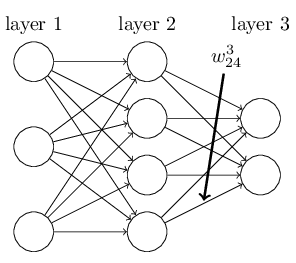
\includegraphics[width=0.4\textwidth]{images/vaha_v_siti.png}
    \caption{Příklad zápisu váhy}\cite{vaha_v_siti}
\end{figure}

Podobná notace se použije také při popisu biasu, neaktivované a aktivované hodnoty neuronu.
Bias neuronu se zapíše jako \(b_{j}^l\), kde \(l\) je vrstva neuronu a \(j\) je \(j\)-tý neuron v \(l\)-té vrstvě.
Hodnota neuronu před aktivací je označí písmenem \(z_{j}^{l} = \left( \sum (w^{l}_{jk} \cdot a^{l-1}_k) + b^l_j \right)\).
Hodnota \(z_j^l\) je tedy součet součinů neunonů z předešlé vrsty a příslušných vah.
Hodnota aktivovaného neuronu ze zapíše jako \(a_j^l = f(z_j^l)\), kde funkce \(f(x)\) je nějaké aktivační funkce,
jako například funkce sigmoid \(\sigma(x)\).

\begin{figure}[h]
    \centering
    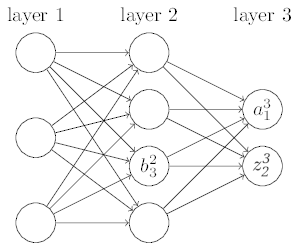
\includegraphics[width=0.4\textwidth]{images/bias_a_neuron.png}
    \caption{Příklad zápisu biasu, aktivace a neaktivace neuronu} \cite{bias_a_neuron}
\end{figure}

Pokud máme upřesněnu notaci, můžeme se posunout k samotnému algoritmu počítání chyby.
Základem, jak už bylo zmíněno, je poměr \(\frac{\delta C}{\delta w}\). Tento vztah je pro výpočet klíčový.
Tento vztah nám vpodstatě říká, jak se změní celková chyba při změně \(w\).

\begin{figure}[h]
    \centering
    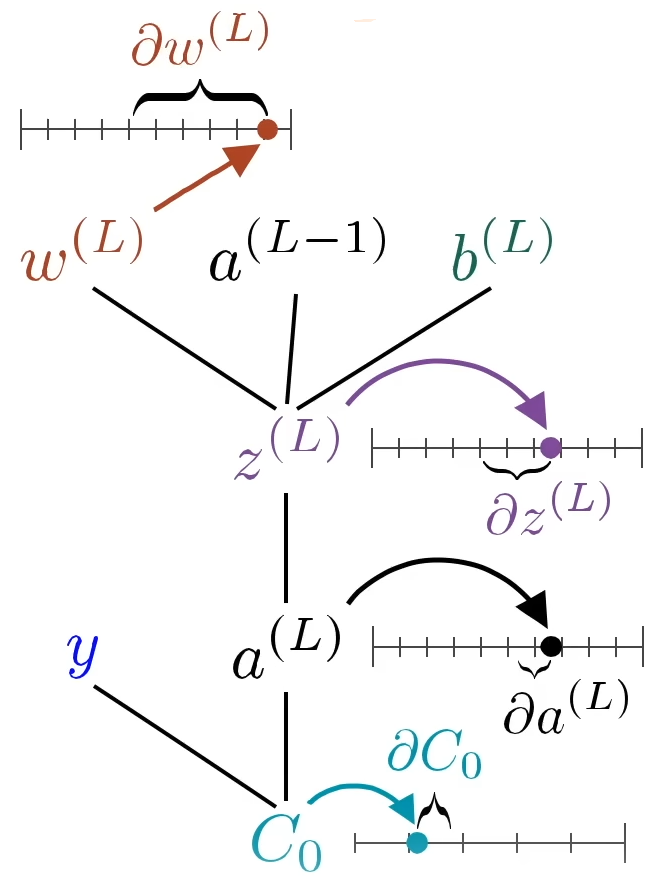
\includegraphics[width=0.35\textwidth]{images/delta.png}
    \caption{Změny} \cite{delta}
\end{figure}

Nejprve si ukážeme pro jednoduchost jak funguje učení neuronové sítě pouze s jedním neuronem na vrstvu. Jak je z obrázku vidět, že když změníme hodnotu \(w^{(L)}\), tak to ovlivní hodnotu \(z^{(L)})\) a to zas nějak ovlivní \(a^{(L)}\) a to pak přímo ovlivní \(C_0\).
Existuje tedy pravidlo, řetězové pravidlo\cite{chain_rule}, které říká, že \(\frac{\delta C_0}{\delta w^{(L)}} = \frac{\delta z^{(L)})}{\delta w^{(L)}} \cdot \frac{\delta a^{(L)}}{\delta z^{(L)}} \cdot \frac{\delta C_0}{\delta a^{(L)}}\).
Toto pravidlo tedy říká, že pokud nějaký prvek nepřímo ovlivňuje poslední prvek, tak se ta změna rovná součinu změně přímo po sobě jdoucích členů.

Jakmile máme tento vztah, je potřeba spočítat derivaci čitatele vůči jmenovateli.

Protože \(C_0 = (a^{(L)} - y)^2\), tak potom bude derivace \(\frac{\delta C_0}{\delta a^{(L)})}= 2(a^{(L)} - y)\).
Parcialní derivace \(\frac{\delta a^{(L)}}{\delta z^{(L)}} = activation'(z^{(L)}) \).
Nakonec parcialní derivace \(\frac{\delta z^{(L)}}{\delta w^{(L)}} = a^{(L-1)}\).
Z toho vyplývá, že \(\frac{\delta C_0}{\delta w^{(L)}} = a^{(L-1)} \cdot activation'(z^{(L)}) \cdot 2(a^{(L)} - y)\)

Už zbývá spočítat chybu vůči vahám, aby byl algoritmus zpětného počítání chyby hotový.
Naštěstí se počítání moc neliší od počítání chyby vůči vahám.
Vzorec pro spočítání zůstane skoro stejný, kde \(\frac{\delta C_0}{b_j^{(L)}} = \frac{\delta z^{(L)})}{\delta b^{(L)}} \cdot \frac{\delta a^{(L)}}{\delta z^{(L)}} \cdot \frac{\delta C_0}{\delta a^{(L)}} \).
Derivace \(\frac{\delta z^{(L)}}{\delta b^{(L)}} = 1 \) a zbytek derivací zůstane stejný. Tedy \(\frac{\delta C_0}{b_j^{(L)}} =  activation'(z^{(L)}) \cdot 2(a^{(L)} - y)\).

Jakmile máme odvozený vztah pro \(\frac{\delta C_0}{\delta w^{(L)}}\), můžeme odvodit pravidlo rozšířit, aby fungovalo obevně pro všechny neuronové sítě.
Tím pádem nás zajímá \(\frac{\delta C_0}{\delta w_{jk}^{(L)}}\). Prvním rozdílem je, že \(C_0 = \sum_{j=1}^{n_L}(a_j^{(L)} - y_j)^2 \).
Druhým rozdílem je, že \(\frac{\delta C_0}{\delta a_j^{(L-1)}}\) se bude počítat trochu složitěji. Protože neuron \(n_j^{(L-1)}\) ovlivňuje chybu skrz několik cest.
Tím pádem \(\frac{\delta C_0}{\delta a_j^{(L-1)}} = \sum_{j=1}^{n_L} \frac{\delta z_j^{(L)}}{\delta a_k^{(L-1)}} \cdot \frac{\delta a_j^{(L)}}{\delta z_j^{(L)}} \cdot \frac{\delta C_0}{\delta a_j^(L)}\)
Z toho vyplývá, že \(\frac{\delta C_0}{\delta a_j^{(L-2)}} = \sum_{j=1}^{n_L} \frac{\delta C_0}{\delta a_j^{(L-1)}} \).

To samé platí i pro výpočet chyby vůči biasu. Tím pádem vzorec pro zůstane stejný a jen s tou změnou, že \(\frac{\delta C_0}{\delta a_j^{(L-2)}} = \sum_{j=1}^{n_L} \frac{\delta C_0}{\delta a_j^{(L-1)}} \).
V tuto chvíli už dokážeme spočítat chybu vůči všem vahám i biasům v síti, a tudíž upravovat jejich hodnoty k lepším.